%%%%%%%%%%%%%%%%%%%%%%%%%%%%%%%%%%%%%%%%%%%%%%%%%%%%%%%%%%%%%%%%%%%%%%
% Lớp 12 | Phương trình mặt phẳng, đường thẳng, mặt cầu | Phương trình đường thẳng trong không gian
% Dạng 2H5?2-6: Khoảng cách điểm tới đường thẳng
% Số câu: 18  (sinh tự động bởi tach_cau.py; từ nay thầy sửa trực tiếp file này)
%%%%%%%%%%%%%%%%%%%%%%%%%%%%%%%%%%%%%%%%%%%%%%%%%%%%%%%%%%%%%%%%%%%%%%

%%%%%%%%%%%%%%%% TRẮC NGHIỆM 4 PHƯƠNG ÁN %%%%%%%%%%%%%%%%

% nguồn: Phan1_Lop_12_Hinh_hoc_Chuong_5
\begin{ex}%[2H5H2-6]%[ma:08120259]
	Trong không gian $Oxyz$, cho điểm $A(1; 2; 3)$. Khoảng cách từ điểm $A$ đến trục  $Ox$ bằng
	 \choice
		 {$\sqrt{4}$}
		{\True  $\sqrt{13}$}
		 {$\sqrt{10}$}
		 {$\sqrt{5}$}
	 \loigiai{
		Trục $Ox$ có  vectơ chỉ phương $\overrightarrow{i}=(1; 0; 0)$.\\
		Khi đó $[\overrightarrow{OA}, \overrightarrow{i}]=(0;  3;-2)$ nên
		\[\mathrm{d}[A, Ox]=\dfrac{|[\overrightarrow{OA},  \overrightarrow{i}]|}{|\overrightarrow{i}|}=\dfrac{\sqrt{3^2+(-2)^2}}{\sqrt{1}}=\sqrt{13}. \]
	} 
\end{ex}

% nguồn: Phan1_Lop_12_Hinh_hoc_Chuong_5
\begin{ex}%[2H5H2-6]%[ma:8b7a62ea]
	Trong không gian với hệ tọa độ $Oxyz$, cho đường thẳng $d$ là giao tuyến của hai mặt phẳng $(P)\colon 2x+y-2z-4=0$ và  $(Q)\colon x-2y+2z+6=0$. Tính khoảng cách $h$ từ điểm $M(1; 0; 1)$ đến đường thẳng $d$.
	 \choice
		{\True $h=3$} 
		{$h=6$} 
		 {$h=9$}
		 {$h=1$}
	\loigiai{ 
		Hai mặt phẳng $(P)\colon 2x+y-2z-4=0$ và $(Q)\colon x-2y+2z-6=0$ có vectơ pháp tuyến  lần lượt là $\overrightarrow{n}_P=(2; 1;-2)$; $\overrightarrow{n}_Q=(1;-2; 2)$.\\
		Giao tuyến $d$ của  hai mặt phẳng $(P)$ và $(Q)$ có vectơ chỉ phương:
		$\overrightarrow{u}=\left[\overrightarrow{n}_P; \overrightarrow{n}_Q\right]=(-2;-6;-5)=-1(2;  6; 5)$.\\
		Đường thẳng  $d$ đi qua $N(0; 2;-1)$, có vectơ chỉ phương $\overrightarrow{u}=(2; 6; 5)$, $\overrightarrow{M N}=(-1; 2;-2)$; $[\overrightarrow{M N}, \overrightarrow{u}]=(22; 1;-10)$.\\
		Khi  đó $\mathrm{d}(M, d)=\dfrac{|[\overrightarrow{MN}, \overrightarrow{u}]|}{|\overrightarrow{u}|}=\dfrac{\sqrt{22^2+1^2+(-10)^2}}{\sqrt{2^2+6^2+5^2}}=3$.
	} 
\end{ex}

% nguồn: Phan1_Lop_12_Hinh_hoc_Chuong_5
\begin{ex}%[2H5H2-6]%[ma:6d1ac885]
	Trong  không gian $Oxyz$, cho mặt phẳng $(\alpha)$ vuông góc với mặt phẳng $(P)\colon x+3y-2z+2=0$ và chứa đường thẳng $d: \dfrac{x-1}{2}=\dfrac{y+1}{-1}=\dfrac{z-4}{1}$. Khoảng cách từ điểm $A(1;-2;-1)$ đến mặt phẳng $(\alpha)$ bằng
	 \choice
		{\True  $\dfrac{8\sqrt{3}}{3}$}
		 {$\dfrac{4\sqrt{3}}{3}$}
		{$\dfrac{24\sqrt{3}}{3}$} 
		 {$8\sqrt{3}$}
	\loigiai{ 
		Ta có $\overrightarrow{n}_{(P)}=(1; 3;-2)$, $\overrightarrow{u}_d=(2;-1; 1) \Rightarrow  \overrightarrow{n}_{(\alpha)}=\left[\overrightarrow{n}_{(P)}; \overrightarrow{u}_d\right]=(1;-5;-7)$.\\
		Điểm $M(1;-1; 4) \in  d \Rightarrow M\in(\alpha)$.\\
		Phương trình mặt phẳng  $(\alpha)$ là $1(x-1)-5(y+1)-7(z-4)=0\Leftrightarrow x-5y-7z+22=0$.\\
		Vậy  $\mathrm{d}(A;(\alpha))=\dfrac{8\sqrt{3}}{3}$.
	 }
\end{ex}

% nguồn: Phan1_Lop_12_Hinh_hoc_Chuong_5
\begin{ex}%[2H5V2-6]%[ma:39c19cee]
	Trong không gian $Oxyz$, cho hai đường thẳng $d_{1}\colon\dfrac{x-2}{6}=\dfrac{y-1}{-1}=\dfrac{z+1}{2}$ và $d_{2}\colon\dfrac{x-1}{3}=\dfrac{y+1}{1}=\dfrac{z+1}{4}$. Gọi $(P)$ là mặt phẳng chứa $d_{2}$ và song song với $d_{1}$. Khoảng cách  giữa $d_{1}$ và $(P)$ là
	 \choice
		{$\dfrac{1}{7}$} 
		 {$2$}
		 {$\dfrac{12}{7}$}
		{\True $1$} 
	 \loigiai{
		Vectơ chỉ phương  của $d_1$ và $d_2$ lần lượt là $\overrightarrow{u}_{1}=(6;-1;2)$, $\overrightarrow{u}_{2}=(3;1;4)$.\\
		Vectơ  pháp tuyến $(P)$ là $\overrightarrow{n}=[\overrightarrow{u}_1,\overrightarrow{u}_2]=(-2;-6;3)$.\\
		Vì $d_{2}\subset(P)$, lấy $A(1;-1;-1)\in  d_{2}\Rightarrow A\in(P)$.\\
		 Phương trình $(P)\colon -2(x-1)-6(y+1)+3(z+1)=0
		 \Leftrightarrow-2x-6y+3z-1=0$.\\
		Chọn $B(2;1;-1)\in d_{1}$\\ 
		 Khi đó $\mathrm{d}(d_{1},(P))=\mathrm{d}(B,(P))=\dfrac{|-2\cdot2-6\cdot1+3\cdot(-1)-1|}{\sqrt{(-2)^2+(-6)^2+3^2}}=1$.
	 }
\end{ex}

% nguồn: Phan1_Lop_12_Hinh_hoc_Chuong_5
\begin{ex}%[2H5V2-6]%[ma:e6b00e81]
	Trong không  gian $Oxyz$, cho $A(0;1;2)$ và $d\colon\dfrac{x-2}{2}=\dfrac{y-1}{2}=\dfrac{z-1}{-3}$. Gọi $(P)$ là mặt phẳng đi qua $A$ và chứa $d$. Khoảng cách từ $M(5;-1;3)$ đến $(P)$ bằng
	\choice 
		 {$5$}
		 {$\dfrac{1}{3}$}
		{\True $1$} 
		{$\dfrac{11}{3}$} 
	 \loigiai{
		Lấy $B(2;1;1)\in d$,  ta có $\overrightarrow{AB}=(2;0;-1)$.\\
		Vectơ chỉ  phương $d$ là $\overrightarrow{n}_d=(2;2;-3)$.\\
		$\overrightarrow{n}_P=\left[\overrightarrow{AB},\overrightarrow{n}_d\right]=(2;4;4)=2(1;2;2)$.\\ 
		Phương trình $(P)\colon x+2y+2z-6=0$.\\ 
		Khoảng cách $\mathrm{d}(M,(P))=\dfrac{|5+2(-1)+2\cdot3-6|}{\sqrt{1^2+2^2+2^2}}=1$. 
	} 
\end{ex}

% nguồn: Phan1_Lop_12_Hinh_hoc_Chuong_5
\begin{ex}%[2H5V2-6]%[ma:a88257e0]
	Trong không gian tọa độ $Oxyz$, cho điểm $A(-3; 1;-3)$ và đường thẳng  $d: \dfrac{x+1}{2}=\dfrac{y-2}{-3}=\dfrac{z}{1}$. Gọi $(\alpha)$ là mặt phẳng chứa đường thẳng $d$ và vuông góc với mặt phẳng tọa độ $(Oyz)$. Khoảng cách từ $A$ đến mặt phẳng $(\alpha)$ bằng
	\choice 
		{$2\sqrt{10}$} 
		{\True  $\sqrt{10}$}
		 {$\dfrac{8\sqrt{10}}{5}$}
		{$\dfrac{4\sqrt{10}}{5}$} 
	 \loigiai{
		Đường thẳng $d$ đi qua điểm $M(-1; 2; 0)$, có  một vectơ chỉ phương $\overrightarrow{u}=(2;-3; 1)$ và mặt phẳng $(Oy z)$ có một vectơ pháp tuyến $\overrightarrow{i}=(1; 0; 0)$.\\
		Do $d \subset(\alpha)$, $(\alpha) \perp(Oyz)$ nên suy ra vectơ $\overrightarrow{n}=[\overrightarrow{u}, \overrightarrow{i}]=(0;-1;-3)$ là  một vectơ pháp tuyến của mặt phẳng $(\alpha)$ và $M\in(\alpha)$.\\
		Mặt phẳng $(\alpha)$ đi qua điểm $M(-1; 2; 0)$ và nhận vectơ $\overrightarrow{n}=(0;-1;-3)$ là vectơ pháp  tuyến có phương trình là $y+3z-2=0$.\\
		Khi đó  khoảng cách từ $A$ đến mặt phẳng $(\alpha)$ bằng $\dfrac{|1+3\cdot (-3)-2|}{\sqrt{1^2+3^2}}=\sqrt{10}$.
	 }
\end{ex}

% nguồn: Phan1_Lop_12_Hinh_hoc_Chuong_5
\begin{ex}%[2H5V2-6]%[ma:2fa3105b]
	Trong không gian $Oxyz$, cho hai đường thẳng $\Delta: \dfrac{x}{2}=\dfrac{y+2}{3}=\dfrac{z}{4}$, $d: \dfrac{x-1}{2}=\dfrac{y-2}{1}=\dfrac{z-1}{2}$. Gọi $(P)$ là mặt phẳng chứa đường thẳng  $\Delta$ và song song với đường thẳng $d$. Tính khoảng cách từ điểm $M(3; 0;-1)$ đến mặt phẳng $(P)$.
	\choice 
		{\True  $3$}
		{$\dfrac{2}{3}$} 
		 {$\dfrac{5}{3}$}
		 {$1$}
	\loigiai{ 
		Đường thẳng $\Delta$ đi  qua điểm $M(0;-2; 0)$ và có vectơ chỉ phương $\overrightarrow{u_{\Delta}}=(2; 3; 4)$.\\
		Đường thẳng  $d$ đi qua điểm $N(1; 2; 1)$ và có vectơ chỉ phương $\overrightarrow{u_d}=(2; 1; 2)$.\\
		Khi đó: $\overrightarrow{n}_P=\left[\overrightarrow{u_{\Delta}};  \overrightarrow{u_d}\right]=(1; 2;-2)$.\\
		Mặt  phẳng $(P)\colon 1(x-0)+2(y+2)-2(z-0)=0\Leftrightarrow x+2y-2z+4=0$.\\
		Thử lại $N\notin(P)$ nên thỏa  mãn.\\
		Vậy  $\mathrm{d}(M;(P))=\dfrac{|3+2\cdot 0-2\cdot (-1)+4|}{\sqrt{1^2+2^2+(-2)^2}}=3$.
	 }
\end{ex}

% nguồn: Phan1_Lop_12_Hinh_hoc_Chuong_5
\begin{ex}%[2H5V2-6]%[ma:c1770f50]
	Cho lăng trụ đứng $ABC.A'B'C'$ có đáy $ABC$ là tam giác vuông tại $B$, $AB=a$, $BC=a\sqrt{2}$, $AA'=a\sqrt{3}$. Trên $BB'$ lấy điểm $N$ sao cho $BN = \dfrac{a}{\sqrt{3}}$. Khoảng cách từ $B'$ đến mặt phẳng $(AC'N)$ bằng 
	\choice 
		{\True  $\dfrac{a\sqrt{6}}{2}$}
		 {$a\sqrt{6}$}
		 {$\dfrac{a\sqrt{6}}{6}$}
		{$\dfrac{a\sqrt{6}}{3}$} 
	 \loigiai{
		\begin{center}
			\begin{tikzpicture}[line join = round,line cap=round,>=stealth,font=\footnotesize,scale=1]
					\path 
						(0,1.5)  coordinate (A)
						 (1.5,0) coordinate (B)
						 (5,1.5) coordinate (C)
						(0,5) coordinate (A') 
						 (1.5,3.5) coordinate (B')
						(5,5) coordinate (C') 
						($(B')! 2/3  !(B)$) coordinate (N);
					\draw  (A)--(B) node[midway,left]{$a$}--(C) node[midway,right]{$a\sqrt{3}$}
						 (A)--(A')
						(B)--(B') 
						(C)--(C') 
						 (A')--(B')--(C')--cycle (A)--(N)--(C')
						(N)--(B)  node[midway,right]{$\dfrac{a}{\sqrt{3}}$};
					 \draw[dashed] (C')--(A)--(C);
					 \draw[->] (A)--(-0.5,2) node[left]{$x$}; \draw[->] (C)--(6,2) node[above]{$y$}; \draw[->] (B')--++(0,3) node[right]{$z$};
					\foreach  \p/\r in {A/180,B/-90,C/-30,A'/90,B'/-40,C'/0,N/-30}
					\fill (\p) circle (1.2pt)  node[shift={(\r:3mm)}]{$\p$};
				\end{tikzpicture}
		\end{center}
		Chọn hệ trục tọa độ như hình vẽ, khi đó  ta có $A(a;0;0)$, $N\left(0;0;\dfrac{a}{\sqrt{3}}\right)$, $C'\left(0;a\sqrt{2};a\sqrt{3}\right)$,
		$B'(0;0;a\sqrt{3})$. $\overrightarrow{AN} = \left(-a;0;\dfrac{a}{\sqrt{3}}\right)$, $\overrightarrow{AC'}  = (-a;a\sqrt{2};a\sqrt{3})$.\\
		Mặt phẳng $(AC'N)$ đi qua $A(a;0;0)$ có vectơ pháp tuyến $\overrightarrow{n}  = \left[\overrightarrow{AN}, \overrightarrow{AC'}\right] = \left(-\dfrac{a^2\sqrt{6}}{3}; \dfrac{2a^2\sqrt{3}}{3}; -a^2\sqrt{2}\right)$ có phương trình
		là $(AC'N)$$\colon$ $-\dfrac{\sqrt{6}}{3}(x-a) +  \dfrac{2\sqrt{3}}{3}y - \sqrt{2}z = 0$.\\
		Khoảng cách $\mathrm{d}\left(B', (AC'N)\right) =  \dfrac{\left|\dfrac{a\sqrt{6}}{3}-a\sqrt{6}\right|}{\sqrt{\dfrac{6}{9}+\dfrac{4}{3}+2}}=\dfrac{a\sqrt{6}}{3}$.
	 }
\end{ex}

% nguồn: Phan1_Lop_12_Hinh_hoc_Chuong_5
\begin{ex}%[2H5V2-6]%[ma:52ef1638]
	Cho  lăng trụ $ABCD.A'B'C'D'$ có đáy $ABCD$ là hình chữ nhật và $AB=a$, $AD=a\sqrt{3}$. Hình chiếu vuông góc của điểm $A$ lên mặt phẳng $(A'B'C'D')$ trùng với giao điểm của $A'C'$ và $B'D'$. Khoảng cách từ điểm $B$ đến $(AB'D')$ bằng
	 \choice
		 {\True $\dfrac{a\sqrt{3}}{2}$}
		 {$\dfrac{a\sqrt{3}}{4}$}
		{$\dfrac{a\sqrt{3}}{3}$} 
		 {$\dfrac{a\sqrt{3}}{6}$}
	\loigiai{ 
		\begin{center}
			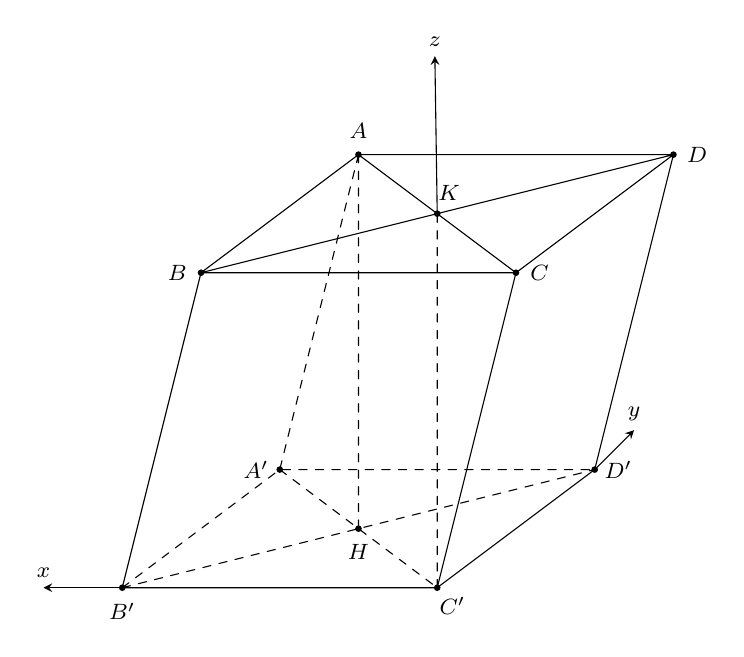
\begin{tikzpicture}[line join = round,line cap=round,>=stealth,font=\footnotesize,scale=1]
					 \path
						(0,0) coordinate (B') 
						(2,1.5) coordinate  (A')
						 (4,0) coordinate (C')
						(6,1.5) coordinate (D') 
						(1,4)  coordinate (B)
						(3,5.5)  coordinate (A)
						 (5,4) coordinate (C)
						 (7,5.5) coordinate (D)
						(intersection of A--C and B--D) coordinate (K) 
						(intersection of A'--C' and B'--D')  coordinate (H);
					\draw (B')--(C')--(D') 
						(A)--(B)--(C)--(D)--cycle  (B')--(B)
						 (C)--(C')
						 (D)--(D')
						 (A)--(C)
						 (B)--(D);
					\draw [dashed] (B')--(A')--(D') 
						(A)--(A') 
						 (A')--(C')
						 (B')--(D')
						 (A)--(H)
						(C')--(K); 
					\draw[->](B')--++(-1,0) node[above]{$x$}; \draw[->](D')--++(0.5,0.5) node[above]{$y$}; \draw[->](K)--++(-0.03,2) node[above]{$z$}; 
					\foreach  \p/\r in {A'/180,B'/-90,C'/-50,D'/0,A/90,B/-180,C/0,D/0,K/60,H/-90}
					\fill (\p)  circle (1.2pt) node[shift={(\r:3mm)}]{$\p$};
				\end{tikzpicture}
		\end{center}
		Gọi $H = A'C' \cap B'D'$ và $K = AC \cap BD$.\\ 
		Chọn hệ tọa độ $Oxyz$ như hình vẽ với $C'\equiv O$, $B' \in Ox$, $D' \in Oy$, $K \in Oz$.\\ 
		Đặt $AH = m >  0$.\\
		Khi đó $B'\left(a\sqrt{3};0;0\right)$, $D'(0;a;0)$, $A'(a\sqrt{3};a;0)$, $H\left(\dfrac{a\sqrt{3}}{2}; \dfrac{a}{2}; 0\right)$, $A\left(\dfrac{a\sqrt{3}}{2}; \dfrac{a}{2}; m\right)$.\\ 
		Ta có $\overrightarrow{B'B} = \overrightarrow{A'A} \Rightarrow B\left(\dfrac{a\sqrt{3}}{2};  -\dfrac{a}{2}; m\right)$.\\
		Mặt  khác $\overrightarrow{B'D'} = \left(-a\sqrt{3}; a; 0\right)$, $\overrightarrow{B'A} = \left(-\dfrac{a\sqrt{3}}{2}; \dfrac{a}{2}; m\right)$ nên $(AB'D')$ có véctơ pháp tuyến là
		$\left[\overrightarrow{B'D'}, \overrightarrow{B'A}\right] = \left( am; \sqrt{3}am; 0\right) $ nên $(AB'D')$  có phương trình $x+\sqrt{3}y-a\sqrt{3}=0$.\\
		Vậy $\mathrm{d}\left(B, (AB'D')\right)  = \dfrac{a\sqrt{3}}{2}$.
	} 
\end{ex}

% nguồn: Phan1_Lop_12_Hinh_hoc_Chuong_5
\begin{ex}%[2H5V2-6]%[ma:4c4b2305]
	Trong không gian $Oxyz$, cho hai đường thẳng $\Delta\colon \heva{&x = 0 \\ &y = 2+t \\ &z = -t }$ và $d\colon \heva{&x = \sqrt{2} \\& y = 1+t' \\ &z  = -1+t'}$. Biết rằng có một hình hộp $ABCD.A'B'C'D'$ thỏa mãn $A$, $C$ cùng thuộc $Ox$, $B$, $C'$ cùng thuộc $\Delta$ và $B'$ cùng thuộc $d$. Thể tích của khối hộp $ABCD.A'B'C'D'$ là
	\choice 
		 {$9\sqrt{2}$}
		{\True  $18\sqrt{2}$}
		 {$9$}
		{$18$} 
	 \loigiai{
		\begin{center}
			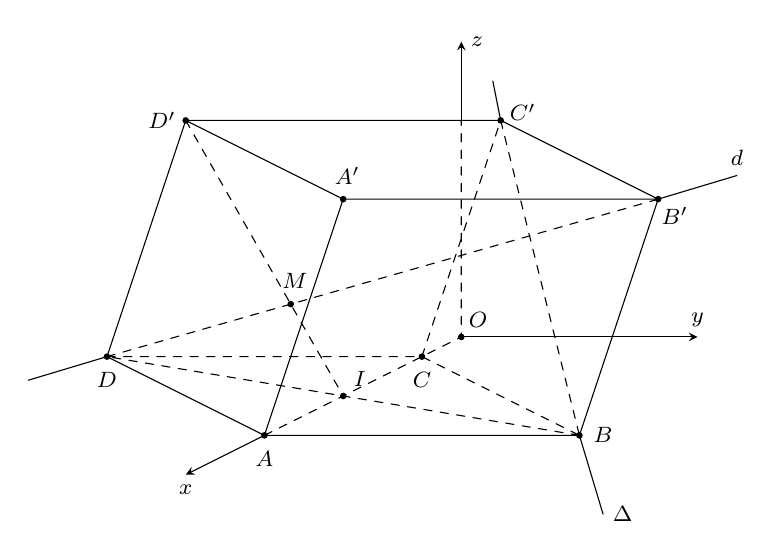
\begin{tikzpicture}[line join = round,line cap=round,>=stealth,font=\footnotesize,scale=1]
					 \path
						 (2,0) coordinate (A)
						(0,1)  coordinate (D)
						 (4,1) coordinate (C)
						(6,0)  coordinate (B)
						(3,3)  coordinate (A')
						(7,3)  coordinate (B')
						 (5,4) coordinate (C')
						(1,4) coordinate (D') 
						(4.5,1.25)  coordinate (O)
						(intersection of  A--C and B--D) coordinate (I)
						(intersection of D'--I and  B'--D) coordinate (M);
					\draw (D)--(A)--(B) 
						(A')--(B')--(C')--(D')--cycle (A)--(A') 
						(B)--(B') 
						 (B)--(B')
						 (D)--(D')
						(D)--++(-1,-0.3) 
						 (B')--++(1,0.3) node[above]{$d$}
						(C')--++(-0.1,0.5) 
						 (B)--++(0.3,-1) node[right]{$\Delta$};
					\draw[->] (4.5,4)--++(0,1)  node[right]{$z$}; \draw[->] (O)--++(3,0) node[above]{$y$}; \draw[->] (A)--++(-1,-0.5) node[below]{$x$};
					\draw[dashed]  (D)--(C)--(B)
						(C)--(C') 
						(C')--(B) 
						(D)--(B') 
						 (A)--(O)--(4.5,4)
						 (B)--(D)
						 (D')--(I);
					\foreach \p/\r  in {A/-90,B/0,C/-90,D/-90,A'/80,B'/-45,C'/20,D'/180,O/45,I/45,M/80}
					\fill  (\p) circle (1.2pt) node[shift={(\r:3mm)}]{$\p$};
				\end{tikzpicture}
		\end{center}
		Nhận xét rằng  các đường thẳng $\Delta$, $d$, $Ox$ đôi một vuông góc với nhau $\heva{&AC \perp BC'\\& BC' \perp B'D' \\ &B'D \perp AC.}$\\
		Gọi $I$ là tâm của hình  bình hành $ABCD$ và $M$ là giao của $D'I$ và $B'D$.\\
		Ta có $\dfrac{IM}{MD'} = \dfrac{IB}{B'D'} = \dfrac{1}{3}  \Rightarrow IM = \dfrac{1}{3}ID'$.\\
		Mặt khác $\heva{&B'D \perp AC \\ &B'D \perp BC'} \Rightarrow B'D \perp AD' \Rightarrow B'D  \perp (AD'C)$.\\
		Kẻ $MH \parallel AD'$ ($H \in AC$) $\Rightarrow MH \perp AC$ suy ra $MH$ là đoạn vuông góc chung của $AC$, $B'D$.\\ $\Rightarrow MH =  \mathrm{d}(AC, B'D) = \mathrm{d}(Ox, d) = \sqrt{2}$.\\
		Vì $\dfrac{MH}{AD'} = \dfrac{IM}{ID'} =  \dfrac{1}{3} \Rightarrow AD' = 3\sqrt{2}$.\\
		Kẻ $MK \parallel AC$  ($K \in AD'$) $\Rightarrow MK \perp AD'$ suy ra $MK$ là đoạn vuông góc chung của $AD', B'D$.\\
		$\Rightarrow MK =  \mathrm{d}(AD', B'D) = \mathrm{d}(\Delta, d) = \sqrt{2}$.\\
		Vì $\dfrac{MK}{AI} = \dfrac{D'M}{D'I} = \dfrac{2}{3} \Rightarrow AI = \dfrac{3\sqrt{2}}{2} \Rightarrow  AC=3\sqrt{2}$.\\
		Ta lại có $BC' \parallel (AD'C) \Rightarrow \mathrm{d}(BC', AC)  = \mathrm{d}\left(BC', (AD'C)\right) = \mathrm{d}\left(B, (AD'C)\right) = \mathrm{d}\left(D, (AD'C)\right)$.\\
		$\Rightarrow \mathrm{d}\left(D,  (AD'C)\right) = \mathrm{d}(Ox, \Delta) = \sqrt{2}$.\\
		$\Rightarrow V_{D.AD'C}  = \dfrac{1}{3}\mathrm{d}\left(D, (AD'C)\right)\cdot S_{AD'C} = \dfrac{1}{3}\mathrm{d}\left(D, ( AD'C)\right)\cdot\dfrac{1}{2}AD'\cdot AC=3\sqrt{2}$.\\
	} 
\end{ex}

% nguồn: Phan1_Lop_12_Hinh_hoc_Chuong_5
\begin{ex}%[2H5V2-6]%[ma:bff5347e]
	Cho lăng trụ $ABC.A'B'C'$ có tam giác $ABC$  đều cạnh bằng $2a$. Hình chiếu vuông góc của $A'$ lên mặt phẳng $(ABC)$ trùng với trung điểm $M$ của $BC$. Biết góc tạo bởi $A'B$ và mặt đáy bằng $60^\circ$. Khoảng cách từ $B$ đến mặt phẳng $(AB'C)$ là
	\choice 
		 {$\dfrac{a\sqrt{7}}{7}$}
		 {$\dfrac{2a\sqrt{7}}{7}$}
		{\True  $\dfrac{2a\sqrt{39}}{13}$}
		{$\dfrac{a\sqrt{39}}{13}$} 
	 \loigiai{
		\begin{center}
			\begin{tikzpicture}[line join = round,line cap=round,>=stealth,font=\footnotesize,scale=1]
					\path 
						(0,1) coordinate (A) 
						(1,0)  coordinate (B)
						(4.5,1) coordinate  (C)
						(2.8,5) coordinate  (A')
						(3.8,4) coordinate  (B')
						 (7.3,5) coordinate (C')
						($(B)! 1/2 !(C)$) coordinate  (M);
					\draw (A)--(B)--(C) 
						(A')--(B')--(C')--cycle  (A)--(A')
						(B)--(B') 
						(C)--(C') 
						(A')--(B); 
					\draw[dashed]  (A)--(C)
						 (A')--(M)--(A);
					\draw[line  width=0.5pt] (A)--(B')--(C);
					\draw[fill=gray!70,dashed,opacity=0.4]  (A)--(B')--(C)--cycle;
					\draw pic[draw,angle radius=3mm] {right angle = A'--M--C}; 
					\draw (M)  node[below right]{$M\equiv O$};
					\draw [->]  (A')--++(0,1) node[right]{$z$}; \draw [->] (A)--++(-1,0.2) node[below]{$x$}; \draw [->] (B)--++(-1,-0.3) node[below]{$y$};
					\foreach \p/\r  in {A/200,B/-90,C/0,A'/130,B'/-30,C'/0}
					\fill (\p)  circle (1.2pt) node[shift={(\r:3mm)}]{$\p$};
				\end{tikzpicture}
		\end{center}
		Góc giữa $A'B$ và mặt phẳng  $(ABC)$ là góc $\widehat{A'BM}=60^{\circ}$.\\
		Ta có $A'M =  BM\cdot\tan 60^{\circ} = a\sqrt{3}$; $AM = AB\cdot\sin 60^{\circ} = 2a\cdot\dfrac{\sqrt{3}}{2} = a\sqrt{3}$.\\
		Đặt hệ trục tọa $Oxyz$ như hình vẽ. Coi $a=1$ khi đó $A(\sqrt{3};0;0)$, $B(0;1;0)$,  $C(0;-1;0)$,
		$A'(0;0;\sqrt{3})$. Gọi $B'(x_0;y_0;z_0)$, $\overrightarrow{A'B'} = (x_0;y_0;z_0-\sqrt{3})$, $\overrightarrow{AB} = (-\sqrt{3};1;0)$.\\ 
		Vì $\overrightarrow{A'B'} = \overrightarrow{AB}$ nên $\heva{&x_0 = -\sqrt{3}\\& y_0  = 1 \\ &z_0=\sqrt{3}} \Rightarrow B'(-\sqrt{3};1;\sqrt{3})$.\\
		Ta có $\heva{&\overrightarrow{AC} =  (-\sqrt{3};-1;0)\\&\overrightarrow{AB'} = (-2\sqrt{3};1;\sqrt{3})} \Rightarrow \left[\overrightarrow{AC}, \overrightarrow{AB'}\right] = (-\sqrt{3};3;-3\sqrt{3}) \Rightarrow \overrightarrow{n}=(1;-\sqrt{3};3)$ là vectơ pháp tuyến của $\mathrm{mp}(ACB')$. \\
		Phương trình mặt phẳng $(ACB')$ là $x-\sqrt{3}y+3z-\sqrt{3}=0$.\\ 
		$\Rightarrow \mathrm{d}\left(B, (ACB')\right)  = \dfrac{\left|0+\sqrt{3}\cdot1+0-\sqrt{3}\right|}{\sqrt{1+3+9}} = \dfrac{2\sqrt{39}}{13}$.\\
		Vậy khoảng cách  từ $B$ đến $(AB'C)$ là $\dfrac{2a\sqrt{39}}{13}$.
	 }
\end{ex}


%%%%%%%%%%%%%%%% ĐÚNG/SAI %%%%%%%%%%%%%%%%

% nguồn: Phan1_Lop_12_Hinh_hoc_Chuong_5
\begin{ex}%[2H5H2-6]%[ma:1507055f]
	 Trong không gian với hệ trục tọa độ $Oxyz$, cho điểm $M(1;2;3)$ và đường thẳng $\Delta\colon\dfrac{x-1}{2}=\dfrac{y}{1}=\dfrac{z+1}{-1}$.
	 \choiceTF
		{Đường thẳng $\Delta$ có một  vectơ chỉ phương là $\overrightarrow{a}=(2;-1;1)$}
		{\True Mặt phẳng $(P)$  qua $M$ và vuông góc với $\Delta$ có phương trình là $2x+y-z-1=0$}
		{\True Mặt cầu  tâm $I(2;2;-1)$ và tiếp xúc với mặt phẳng $(P)$ có phương trình $(x-2)^2+(y-2)^2+(z+1)^2=6$}
		{Khoảng cách từ điểm $M$ đến  đường thẳng $\Delta$ là $5$}
	\loigiai{ 
	\begin{itemchoice}
		\itemch Đường  thẳng $\Delta$ có một vectơ chỉ phương là $\overrightarrow{u} = (2;1;-1)$.\\
		Do $\overrightarrow{a} = (2;-1;1)$ không cùng phương với $\overrightarrow{u}$ nên $\overrightarrow{a}$ không là vectơ chỉ phương của $\Delta$. 
		\itemch Do mặt phẳng $(P)$ vuông góc với đường thẳng $\Delta$ nên nhận $\overrightarrow{u} = (2;1;-1)$ là một  vectơ pháp tuyến.\\
		Phương trình mặt phẳng $(P)$ đi qua điểm $M(1;2;3)$ nhận $\overrightarrow{u} = (2;1;-1)$  là vectơ pháp tuyến là
		\begin{eqnarray*}
			&& 2(x - 1) +  1(y - 2) - 1(z - 3) = 0 \\
			&\Leftrightarrow& 2x + y - z - 1 =  0.
		\end{eqnarray*}
		\itemch Bán kính mặt cầu tâm $I(2;2;-1)$ và tiếp xúc với mặt phẳng  $(P)$ là
		\[R=\mathrm{d}\left(I,(P)\right)=\dfrac{|2\cdot2+2+1-1|}{\sqrt{2^2+1^2+(-1)^2}}=\sqrt{6}.\] 
		Suy ra mặt cầu có phương trình là  $(x-2)^2+(y-2)^2+(z+1)^2=6$.
		\itemch Khoảng cách từ điểm $M$ đến đường thẳng $\Delta$ có $A(1;0;-1)\in\Delta$ và vectơ chỉ phương $\overrightarrow{u}=(2;1;-1)$  bằng
		\[\mathrm{d}(M,\Delta)=\dfrac{\left|\left[\overrightarrow{AM},\overrightarrow{u}\right]\right|}{\left|\overrightarrow{u}\right|}=\dfrac{\sqrt{(-6)^2+8^2+(-4)^2}}{\sqrt{2^2+1^2+(-1)^2}}=\dfrac{\sqrt{174}}{3}\approx  4{,}4.\]
	\end{itemchoice}
	 }
\end{ex}

% nguồn: Phan1_Lop_12_Hinh_hoc_Chuong_5
\begin{ex}%[2H5H2-6]%[ma:b6039819]
	Trong không gian với hệ trục $Oxyz$ cho điểm $M(1;2;3)$ và  đường thẳng $\Delta\colon\dfrac{x-1}{2}=\dfrac{y}{1}=\dfrac{z+1}{-1}$.
	\choiceTF 
		{Đường thẳng $\Delta$ có  một vectơ chỉ phương là $\overrightarrow{a}=(2;-1;1)$}
		{\True Mặt phẳng $(P)$ qua  $M$ và vuông góc với $\Delta$ có phương trình là $2x+y-z-1=0$}
		{\True Mặt cầu tâm $I(2;2;-1)$  và tiếp xúc với mặt phẳng $(P)$ có phương trình $(x-2)^2+(y-2)^2+(z+1)^2=6$}
		{Khoảng cách từ điểm $M$  đến đường thẳng $\Delta$ là $5$}
	 \loigiai{
	\begin{itemchoice}
		\itemch Đường thẳng $\Delta$ nhận vectơ chỉ phương có  dạng $\overrightarrow{a}=k(2;-1;-1)$, với $k\in\mathbb{Z}$.
		\itemch Mặt phẳng $(P)\colon 2x+y-z-1=0$ có vectơ  pháp tuyến là $\overrightarrow{n}=(2;1;-1)$. \\
		$\Rightarrow \overrightarrow{a}\parallel\overrightarrow{n} \Rightarrow  (P)\perp(\Delta)$.
		\itemch  Bán kính mặt cầu tâm $I(2;2;-1)$ và tiếp xúc với mặt phẳng $(P)$ là
		\[R=\mathrm{d}(I,(P))=\dfrac{|2\cdot2+2+1-1|}{\sqrt{2^2+1^2+(-1)^2}}=\sqrt{6}.\] 
		Suy ra mặt cầu  có phương trình là $(x-2)^2+(y-2)^2+(z+1)^2=6$.
		\itemch Khoảng cách từ điểm $M$ đến  đường thẳng $\Delta$ có $A(1;0;-1)\in\Delta$ và vectơ pháp tuyến $\overrightarrow{n}=(2;1;-1)$ bằng
		\[\mathrm{d}(M,\Delta)=\dfrac{\left|\left[\overrightarrow{AM},\overrightarrow{n}\right]\right|}{\left|\overrightarrow{n}\right|}=\dfrac{\sqrt{(-6)^2+8^2+(-4)^2}}{\sqrt{2^2+1^2+(-1)^2}}=\dfrac{\sqrt{174}}{3}\approx  4{,}4.\]
	\end{itemchoice}
	} 
\end{ex}

% nguồn: Phan1_Lop_12_Hinh_hoc_Chuong_5
\begin{ex}%[2H5V2-6]%[ma:46e069af]
	 Trong không gian với hệ trục tọa độ $Oxyz$, một tàu ngầm đang di chuyển dưới biển sâu với hướng di chuyển theo đường thẳng $\Delta\colon\dfrac{x-50}{3}=\dfrac{y+20}{-4}=\dfrac{z-10}{1}$. Hải quân phát hiện một khu vực nguy hiểm được rải mìn, khu vực này có dạng hình cầu $(S)$ với tâm $C(200;-300;60)$ và bán kính $R=80$ (đơn vị đo là mét).
	 \choiceTF
		{\True Một véc-tơ chỉ phương  của đường thẳng $\triangle$ là $(3;-4; 1)$}
		{\True Đường di chuyển $\Delta$ nằm trong mặt phẳng $(P)\colon 4x+3y=140$} 
		{Tàu ngầm sẽ không đi  vào khu vực nguy hiểm $(S)$}
		{\True Gọi $M$ là điểm gần khu vực mìn nhất trên đường đi của tàu ngầm. Biết rằng tốc độ tàu ngầm  không đổi là $5$ (m/s). Thời gian ngắn nhất để tàu ngầm di chuyển từ vị trí hiện tại $A(50;-20;10)$ đến điểm $M$ là $51$ giây (Kết quả làm tròn đến hàng đơn vị)}
	 \loigiai{
		\begin{itemchoice}
			 \itemch \textbf{Đúng}. Đường thẳng $\Delta\colon\dfrac{x-50}{3}=\dfrac{y+20}{-4}=\dfrac{z-10}{1}$ có một véc-tơ chỉ phương là $(3;-4; 1)$.
			\itemch \textbf{Đúng}. Ta có điểm  $A(50;-20;10) \in \Delta$.\\
			Mặt khác thay  tọa độ điểm $A$ vào phương trình mặt phẳng $(P)$ ta được\\ $4\cdot 50+3\cdot (-200)-140=0$ nên điểm $A \in (P)$.\\
			Dễ thấy véc-tơ pháp tuyến của $(P)$ là  $\overrightarrow{n}_{(P)}=(4;3;0)$ và $\overrightarrow{u}_{\Delta}$ vuông góc với nhau nên đường thẳng $\Delta$ nằm trong mặt phẳng $(P)$.
			\itemch \textbf{Sai}. Ta có  $A(50;-20;10) \Rightarrow \overrightarrow{AC}=(150;-280;50)$ nên $\left[\overrightarrow{u}_{\Delta},\overrightarrow{AC}\right]=(80;0;-240)$.\\
			Khoảng cách từ điểm $C$ đến  đường thẳng $\Delta$ là
			\begin{eqnarray*}
				d_{(C,\Delta)}=\dfrac{\left[\overrightarrow{u}_{\Delta},\overrightarrow{AC}\right]}{|\overrightarrow{u}_{\Delta}|}=\dfrac{80\sqrt{65}}{13}\approx 49{,}6<R=80. 
			\end{eqnarray*}
			Vậy tàu ngầm sẽ đi vào khu vực nguy hiểm. 
			\itemch \textbf{Đúng}. \begin{center}
			\begin{tikzpicture}[smooth,line join=round,line cap=round,font=\footnotesize,scale=.6]
					\path 
						(0,0) coordinate (C) node[below]{$C$} 
						(-4,3) coordinate  (P) node[above]{$P$}
						(-6,3) coordinate  (A) node[left]{$A$}
						(6,3) coordinate (B) node[above]{$\Delta$} 
						 (0,3) coordinate (M) node[above]{$M$};
					 \draw (C) circle (5cm);
					\draw (A)--(B) 
						 (C)--(M)
						(C)--(P); 
					 \foreach \i in {(A),(C),(M),(P)} \draw[fill] \i circle (2pt);
				\end{tikzpicture}
		\end{center}
		Điểm $M  \in \Delta$ suy ra $M(50+3t;-20-4t;10+t)$ và $\overrightarrow{CM}=(3t-150;-4t+280;t-50)$.\\
		Lại  có
		\begin{eqnarray*}
			&&\overrightarrow{CM} \perp  \overrightarrow{u}_{\Delta}\\
			&\Rightarrow& (3t-150)\cdot 3+(-4t+280)\cdot (-4)+(t-150)\cdot  1=0\\
			&\Leftrightarrow& 26t-1620=0  \\
			 &\Leftrightarrow& t=\dfrac{810}{13}.
		\end{eqnarray*}
		Vậy $M\left(\dfrac{3080}{13};-\dfrac{3500}{13}; \dfrac{940}{13} \right)$  nên khoảng cách từ điểm $A$ đến điểm $M$ là $AM=\dfrac{810\sqrt{26}}{13}$\,m.\\
		Mặt  khác $CM=\dfrac{80\sqrt{65}}{13}$\,m.\\
		Suy  ra $MP=\sqrt{R^2-CM^2}=\sqrt{80^2-\left(\dfrac{80\sqrt{65}}{13}\right)^2}=\dfrac{160\sqrt{26}}{13}$.\\
		Do đó $AP=AM-MP=\dfrac{80\sqrt{26}}{13}-\dfrac{160\sqrt{26}}{13}=50\sqrt{26}$.\\ 
		Vậy thời  gian ngắn nhất để tàu ngầm di chuyển từ vị trí hiện tại $A(50;-20;10)$ đến điểm $M$ là
		 $t_{\min}=\dfrac{AP}{v}=\dfrac{50\sqrt{26}}{5}\approx 51$ giây.
	\end{itemchoice}
 }
\end{ex}

% nguồn: Phan1_Lop_12_Hinh_hoc_Chuong_5
\begin{ex}%[2H5V2-6]%[ma:38ce6511]
	Trong không  gian $Oxyz$, cho hai đường thẳng $(d_{1})\colon \dfrac{x-1}{2}=\dfrac{y-2}{5}=\dfrac{z-3}{1}$ và $(d_{2})\colon
	\heva{& 
	 x=t \\&
	 y=1+t \\&
	 z=2+t}$.
	 \choiceTF
		{\True Điểm $B(-2;-1;0)$ thuộc  đường thẳng $(d_{2})$}
		{\True Một  vectơ chỉ phương của $(d_{1})$ là $\overrightarrow{a}=(-2;-5;-1)$}
		{Hai đường thẳng $(d_{1})$ và $(d_{2})$ là hai đường thẳng chéo  nhau}
		{\True Gọi $M (a; b; c)$ là điểm thuộc $(d_{2})$ sao cho độ dài $OM$ là  ngắn nhất. Khi đó $a+b+c=0$}
	 \loigiai{
		\begin{itemchoice}
			\itemch Đúng.\\ 
			Thay tọa độ điểm $B(-2;-1;0)$ vào phương trình  của $d_2$ ta được
			$$\heva{& 
			-2=t  \\&
			 -1=1+t \\&
			0=2+t}\Leftrightarrow  \heva{&
			t=-2 \\& 
			 t=-2 \\&
			t=-2}\Leftrightarrow t=-2.$$ 
			\itemch  Đúng.\\
			Đường thẳng $(d_{1})$  có phương trình là $ \dfrac{x-1}{2}=\dfrac{y-2}{5}=\dfrac{z-3}{1}$ nên có một vectơ chỉ phương là $\overrightarrow{u}=(2;5;1)$.\\
			Vì $\overrightarrow{a}(-2;-5;-1)$ và $\overrightarrow{u}(2;5;1)$ cùng phương nên $\overrightarrow{a}(-2;-5;-1)$ cũng là  một vectơ chỉ phương của đường thẳng $(d_1)$.
			\itemch  Sai.\\
			Đường thẳng $(d_1)$ đi qua $M(1;2;3)$, có vectơ chỉ phương là $\overrightarrow{u}=(2;5;1)$; đường thẳng $(d_2)$ đi qua $N(0;1;2)$, có vectơ chỉ phương là $\overrightarrow{v}=(1;1;1)$.\\ 
			Vì $\overrightarrow{u}(2;5;1)$ và $\overrightarrow{v}(1;1;1)$ đồng thời $[\overrightarrow{u},\overrightarrow{v}]\cdot \overrightarrow{MN}=0$ nên hai đường thẳng $(d_1)$ và $(d_2)$  cắt nhau.
			 \itemch Đúng.\\
			Vì điểm $M$ thuộc đường thẳng $d_2$ nên giả sử $M(t;1+t;2+t)$ với $t\in \mathbb{R}$.\\ 
			Ta có $$OM=\sqrt{t^2+(1+t)^2+(2+t)^2}=\sqrt{3(t+1)^2+2}\ge \sqrt{2}.$$ 
			Đẳng thức xảy ra khi và chỉ  khi $t=1$, tức là khi $M(-1;0;1)$.\\
		\end{itemchoice}
	} 
\end{ex}


%%%%%%%%%%%%%%%% TRẢ LỜI NGẮN %%%%%%%%%%%%%%%%

% nguồn: Phan2_Lop_12_Hinh_hoc_Chuong_5
\begin{bt}%[2H5V2-6]%[ma:c3d3e7df]
	Trong không gian với hệ tọa độ $Oxyz$, cho điểm $A(3;-1;0)$ và đường thẳng $d\colon\dfrac{x-2}{-1}=\dfrac{y+1}{2}=\dfrac{z-1}{1}$. Biết mặt phẳng $(\alpha)\colon ax+by-z=0$ chứa $d$ sao  cho khoảng cách từ A đến $(\alpha)$ lớn nhất. Tính giá trị $a+b$.
	\shortans{2} 
	\loigiai{Gọi $H$ là hình chiếu của A đến $d$. Khi  đó $H(2-t;-1+2t;1+t) \Rightarrow \overrightarrow{AH}=(-1-t;2t;1+t)$.\\
		Do $\overrightarrow{AH} \perp d \Rightarrow -1\cdot(-1-t) +2\cdot2t+1\cdot t=0 \Leftrightarrow t=-\dfrac{1}{3}$. Khi đó  $\overrightarrow{AH}=\left(-\dfrac{2}{3};-\dfrac{2}{3};\dfrac{2}{3} \right)$.\\
		Mặt phẳng $(\alpha)$ chứa $d$ sao  cho khoảng cách từ A đến $(\alpha)$ lớn nhất khi $\overrightarrow{AH} \perp(\alpha)$.\\
		Do đó $(\alpha)$ có vectơ pháp tuyến là $\overrightarrow{n}=(1;1;-1)$.\\ Vậy $(\alpha)\colon  1(x-2) +1(y+1) -1(z-1) = 0 \Leftrightarrow x+y-z=0$.\\
	Vậy  $a+b=2$.}
\end{bt}


%%%%%%%%%%%%%%%% TỰ LUẬN %%%%%%%%%%%%%%%%

% nguồn: Phan2_Lop_12_Hinh_hoc_Chuong_5
\begin{bt}%[2H5V2-6]%[ma:71b6c0e9]
	Trong không gian $Oxyz$, khoảng cách giữa đường thẳng $\Delta: \dfrac{x-1}{2}=\dfrac{y+2}{1}=\dfrac{z-1}{2}$ và mặt phẳng $(P)\colon 2x-2y-z+1=0$  bằng bao nhiêu?
	\loigiai{ 
		Đường thẳng $\Delta$ đi qua điểm $M(1;-2; 1)$,  có 1 vectơ chỉ phương $\overrightarrow{u}=(2; 1; 2)$.\\
		Mặt phẳng  $(P)$ có 1 vectơ pháp tuyến $\overrightarrow{n}=(2;-2;-1)$.\\
		Ta có $\overrightarrow{u} \cdot \overrightarrow{n}=2\cdot 2-2\cdot 1-1\cdot  2=0\Rightarrow \overrightarrow{u} \perp \overrightarrow{n}$.\\
		 Mà $M\notin(P) \Rightarrow d \parallel(P) \Rightarrow \mathrm{d}(\Delta,(P))=\mathrm{d}(M,(P))=\dfrac{|2\cdot 1-2\cdot(-2)-1\cdot 1+1|}{\sqrt{2^2+(-2)^2+(-1)^2}}=\dfrac{6}{3}=2$.
	 }
\end{bt}

% nguồn: Phan2_Lop_12_Hinh_hoc_Chuong_5
\begin{bt}%[2H5V2-6]%[ma:ba7f9ffa]
	Trong không gian với hệ trục tọa độ $Oxyz$, cho mặt phẳng $(\alpha): x+y-2z+2=0$ và hai điểm $A(2; 0; 1), B(1; 1; 2)$. Gọi $d$ là đường thẳng nằm trong $(\alpha)$  và cắt đường thẳng $AB$, thỏa mãn góc giữa hai đường thẳng $AB$ và $d$ bằng góc giữa đường thẳng $AB$ và mặt phẳng ($\alpha$). Khoảng cách từ điểm $A$ đến đường thẳng $d$ bằng
	 \loigiai{
		Gọi $A'$  là hình chiếu của $A(2; 0; 1)$ lên $(\alpha)$.\\
		Ta có $B\in(\alpha)$. Gọi $d$ là đường thẳng nằm trong $(\alpha)$ và cắt đường thẳng $AB$, thỏa mãn  góc giữa hai đường thẳng $AB$ và $d$ bằng góc giữa đường thẳng $AB$ và mặt phẳng $(\alpha)$.\\
		 Khi đó $d \equiv A' B\Rightarrow \mathrm{d}(A, d)=\mathrm{d}(A,(\alpha))=\left|\dfrac{2}{\sqrt{6}}\right|=\dfrac{\sqrt{6}}{3}$.
	} 
\end{bt}
